\documentclass[../mathNotesPreamble]{subfiles}

\begin{document}
%  \relscale{1.4} %TODO
  \section{2.1: Functions and Their Graphs}
  \begin{defn*}
    A \textbf{function} is a rule that assigns to each element in a set $A$ one and only one element in a set $B$.

    In the context above, the set $A$ is called the \textbf{domain}, and the set $B$ is called the \textbf{range}.
  \end{defn*}


  \noindent
  \begin{minipage}{0.495\linewidth}
    \centering
    %bottom left corner is (0,0)
    %a,b,c are widths representing left wall to chute, width of chute, chute to right wall
    %h is height of rectangle
    %dx, dy control slope of "funnel"
    %vert is the height of straight parts of "funnel"
    %paths start at top left (on "funnel")
    \begin{tikzpicture}[declare function={
      a=1.25; b=1.25; c=5.5;
      dx=0.9*a; dy=0.6*a;
      h=1.75; vert=0.6;}]
      \path[fill=lander_blue!25, rounded corners=8pt]
        (a-dx,h+2*vert+dy) --++(0,-vert) --++(dx,-dy) |-(0,h)
        --(0,0) -| (c,-vert) --++(-dx, -dy) [sharp corners] --++(0,-vert) %bottom left portion
        --++(b+2*dx,0) [rounded corners=8pt] -- ++(0,vert) --++ (-dx,dy) |- (a+b+c,0)
        --++(0,h) -| (a+b,h+vert) --++(dx,dy) [sharp corners]--++(0,vert) --cycle; %top right portion
      \draw[line width=1pt, rounded corners=8pt]
        (a-dx,h+2*vert+dy) --++(0,-vert) --++(dx,-dy) |-(0,h)
        --(0,0) -| (c,-vert) --++(-dx, -dy) --++(0,-vert) %bottom left portion
        ++(b+2*dx,0) --++(0,vert) --++(-dx,dy) |- (a+b+c,0)
        --++(0,h) -| (a+b,h+vert) --++(dx,dy) --++(0,vert); %top right portion
      \node (Input) [align=center] at ({a+b/2},{h+vert+dy}) {Input\\$x$};
      \node[align=center] at ({(a+b+c)/2},{h/2}) {$f$};
      \node (Output) [align=center] at ({c+b/2},{-vert-dy}) {$f(x)$\\Output};

      \draw[->] (Input) -- ++(0,-vert-dy);
      \draw[<-] (Output) -- ++(0,vert+dy);
    \end{tikzpicture}
  \end{minipage}\hfill%
  \begin{minipage}{0.495\linewidth}
    \begin{center}
      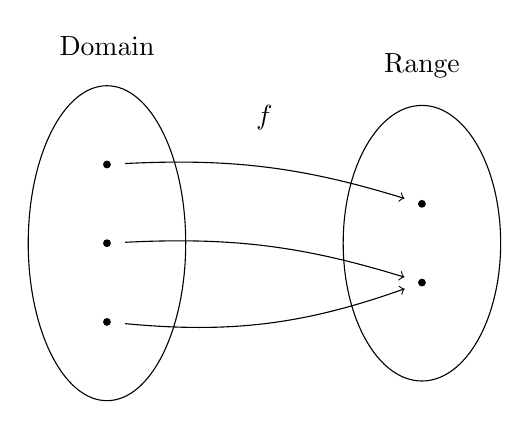
\begin{tikzpicture}
        \draw (-2,0) circle [x radius=1, y radius=2];
        \node at (-2,2.5) {Domain};
        \draw (2,0) circle [x radius=1, y radius=1.75];
        \node at (2,2.25) {Range};
        \node[circle, fill, inner sep=1pt] (xo) at (-2,1) {}; %, label=above:$x_1$
        \node[circle, fill, inner sep=1pt] (fxo) at (2,0.5) {}; %, label=above:$f(x_1)$
        \node[circle, fill, inner sep=1pt] (xt) at (-2,0) {}; %, label=above:$x_2$
        \node[circle, fill, inner sep=1pt] (xr) at (-2,-1) {}; %, label=above:$x_3$
        \node[circle, fill, inner sep=1pt] (fxt) at (2,-0.5) {}; %, label=above:$f(x_2)$
        \node at (0,1.6) {$f$};
        \draw[->, shorten >=5pt, shorten <=5pt] (xo) to [bend left=10] (fxo);
        \draw[->, shorten >=5pt, shorten <=5pt] (xt) to [bend left=10] (fxt);
        \draw[->, shorten >=5pt, shorten <=5pt] (xr) to [bend right=12.5] (fxt);
      \end{tikzpicture}
    \end{center}
  \end{minipage}

  \begin{ex*}
    Let $f(x)=2x^2-2x+1$. Evaluate the following
  \end{ex*}
  \begin{extasks}[after-item-skip=\stretch{1}](2)
    \task $f(1)$
    \task $f(-2)$
    \task $f(a)$
    \task $f(a+h)$
  \end{extasks}
  \vspace*{\stretch{1}}
  \pagebreak

  \begin{ex*}
    Find the domain and range of the following functions:
  \end{ex*}
  \begin{extasks}[after-item-skip=\stretch{1}](2)
    \task $f(x)=x$
    \task $A=\pi r^2$
    \task $y=\sqrt{x-1}$
    \task $y=\dfrac{1}{x^2-4}$
  \end{extasks}
  \vspace*{\stretch{1}}
  \pagebreak

  \begin{defn*}[Vertical Line Test]
    A curve in the $xy$-plane is the graph of a function $y=f(x)$ (an explicit function) if and only if each vertical line intersects it in at most one point
  \end{defn*}
  \begin{ex*}
    Use the vertical line test on the following graphs to determine which graphs may represent an explicit function:
  \end{ex*}

  \begin{center}
    \begin{tabular}{c@{\hspace*{40pt}}c}
      \begin{tikzpicture}[declare function={
        f(\x)=(\x-1.5)*(\x+1)*(\x+2)+6;}]
        \begin{axis}[
          axis lines=center,
          axis line style={black,->},
          xmajorticks=false,
          ymajorticks=false,
          xmin=-3.25, xmax=3.25,
          enlargelimits={value=0.025, auto},
          ticklabel style={font=\footnotesize,inner sep=0.5pt,fill=white,opacity=1.0, text opacity=1},
          xlabel=$x$, xlabel style={at={(ticklabel* cs:1)},anchor=north west},
          ylabel=$y$, ylabel style={at={(ticklabel* cs:1)},anchor=south west},
          every axis plot/.append style={domain=xmin:xmax, line width=0.95pt, color=lander_blue, samples=255},
          ]
          \addplot[<->] expression[domain=-3:2.25]{f(x)};
        \end{axis}
      \end{tikzpicture} &
      \begin{tikzpicture}
        \begin{axis}[
          axis lines=center,
          axis line style={black,->},
          xmajorticks=false,
          ymajorticks=false,
          xmin=-4, xmax=4,
          ymin=-1, ymax=5,
          enlargelimits={value=0.025, auto},
          ticklabel style={font=\footnotesize,inner sep=0.5pt,fill=white,opacity=1.0, text opacity=1},
          xlabel=$x$, xlabel style={at={(ticklabel* cs:1)},anchor=north west},
          ylabel=$y$, ylabel style={at={(ticklabel* cs:1)},anchor=south west},
          every axis plot/.append style={domain=xmin:xmax, line width=0.95pt, color=lander_blue, samples=255},
          ]
          \draw[samples=255, line width=0.95pt, lander_blue, domain=0.2:3.8, <->] plot({(\x-1)*(\x-2)*(\x-3)},{\x});
        \end{axis}
      \end{tikzpicture}\\[2\baselineskip]
      \begin{tikzpicture}[declare function={
        f(\x)=sqrt(\x^2-1);}]
        \begin{axis}[
          axis lines=center,
          axis line style={black,->},
          xmajorticks=false,
          ymajorticks=false,
          ymax=10,
          enlargelimits={value=0.025, auto},
          ticklabel style={font=\footnotesize,inner sep=0.5pt,fill=white,opacity=1.0, text opacity=1},
          xlabel=$x$, xlabel style={at={(ticklabel* cs:1)},anchor=north west},
          ylabel=$y$, ylabel style={at={(ticklabel* cs:1)},anchor=south west},
          every axis plot/.append style={domain=xmin:xmax, line width=0.95pt, color=lander_blue, samples=255},
          ]
          \addplot[<-] expression[domain=-5:-1]{f(x)};
          \addplot[->] expression[domain=1:5]{f(x)};
        \end{axis}
      \end{tikzpicture}&
      \begin{tikzpicture}[declare function={
        g(\x)=1.25*(abs(\x)-1);
        f(\x)=g(\x)<=0 ? sqrt(1-x^2) : g(\x);}]
        \begin{axis}[
          axis lines=center,
          axis equal,
          axis line style={black,->},
          xmajorticks=false,
          ymajorticks=false,
          enlargelimits={value=0.025, auto},
          ticklabel style={font=\footnotesize,inner sep=0.5pt,fill=white,opacity=1.0, text opacity=1},
          xlabel=$x$, xlabel style={at={(ticklabel* cs:1)},anchor=north west},
          ylabel=$y$, ylabel style={at={(ticklabel* cs:1)},anchor=south west},
          every axis plot/.append style={domain=xmin:xmax, line width=0.95pt, color=lander_blue, samples=255},
          ]
          \addplot[<->] expression[domain=-2:2, samples=511]{f(x)};
        \end{axis}
      \end{tikzpicture}
    \end{tabular}
  \end{center}

  \pagebreak
\end{document}
